% В этом шаблоне используется класс spbau-diploma. Его можно найти и, если требуется, 
% поправить в файле spbau-diploma.cls
\documentclass{spbau-diploma}
\usepackage{graphicx}
\usepackage{amsmath}
\begin{document}
% Год, город, название университета и факультета предопределены,
% но можно и поменять.
% Если англоязычная титульная страница не нужна, то ее можно просто удалить.
\filltitle{ru}{
    chair              = {\ },
    title              = {\textbf{ВЫПУСКНАЯ КВАЛИФИКАЦИОННАЯ РАБОТА\\(БАКАЛАВРСКАЯ РАБОТА)}\vskip 0.5 em на тему \vskip 0.5 em\textbf{«Методы оценки сложности текстовых данных для ускорения обучения языковых моделей с помощью обучения по плану»}\\\textit{\small Направление подготовки 01.03.02 Прикладная математика и информатика}},
    % Здесь указывается тип работы. Возможные значения:
    %   coursework - Курсовая работа
    %   diploma - Диплом специалиста
    %   master - Диплом магистра
    %   bachelor - Диплом бакалавра
    % type               = {diploma},
    position           = {студента},
    group              = {БПМ171С},
    author             = {Сурков Максим Константинович},
    supervisorPosition = {?},
    supervisor         = {Ямщиков Иван Павлович},
    reviewerPosition   = {ст. преп.},
    reviewer           = {Привалов А.\,И.},
    % chairHeadPosition  = {д.\,ф.-м.\,н., профессор},
    % chairHead          = {Омельченко А.\,В.},
    university = {\textbf{Федеральное государственное автономное образовательное учреждение высшего образования\\«Национальный исследовательский университет\\«Высшая школа экономики»}},
    faculty = {Факультет Санкт-Петербургская школа физико-математических и компьютерных наук\\Департамент информатики},
    city = {Санкт-Петербург},
    year = {2021}
}
\maketitle

\tableofcontents
\section*{Аннотация}
\ 

Современные системы обработки естественного языка активно используют глубокие нейронные сети (BERT, GPT-3), которые требуют значительных ресурсов для их обучения. За последние годы было разработано множество подходов для решения данной проблемы. Одним из них является обучение по плану. Данный метод состоит из двух составляющих: оценки сложности тренировочных данных и алгоритма их семплирования. Основной целью данной работы является исследование метрик оценки сложности текстовых данных в контексте обучения по плану и влияния данного метода ускорения обучения на скорость сходимости языковых моделей на задачах предобучения и классификации. В процессе исследований было предложено и адаптировано несколько подходов из разных областей математики. Также были реализованы производительные алгоритмы вычисления найденных метрик на больших объемах данных в несколько десятков миллинов тренировочных примеров. Объемный набор экспериментов на задачах предобучения и классификации  выявил наиболее эффективные метрики для использования в обучении по плану. В то же время было установлено, что обучение по плану негативно влияет на скорость сходимости на задаче предобучения, однако не уступает базовому подходу (обучению без плана) на задаче классификации. Также был рассмотрен важный частный случай обучения языковой модели на шумном наборе тренировочных данных. Сравнительный анализ показал ускорение обучения до двух раз на первых 10\% обучения при применении обучения по плану с наиболее эффективной метрикой.
\\

Ключевые слова: обработка естественного языка, обучение по плану, теория информации, оценка сложности текстовых данных

\pagebreak

Modern state-of-the-art natural language processing systems use deep neural networks (BERT, GPT-3) that require many resources for training. Several techniques have been developed for the last ten years. One of them is curriculum learning, which consists of two parts, namely data complexity evaluation and sampling. The main purpose of this work is to research metrics of text complexity in the context of curriculum learning and explore the influence of curriculum learning on training time on pre-training and classification tasks. Several approaches from different mathematics fields were suggested and adapted during the research. Moreover, efficient algorithms for calculating given metrics on large datasets of several tens of millions of samples were implemented. Extensive experiments highlighted the most efficient metrics for use in curriculum learning. At the same time, it was established that curriculum learning negatively affects convergence time on pre-training task, but not inferior to the basic solution (learning without curriculum) on the classification task. Also, training on a noisy training dataset was considered. Comparative analysis showed a double reduction in training time on the first 10\% of training using curriculum learning with the most effective metric.

Keywords: natural language processing, curriculum learning, information theory, text complexity estimation
\section*{Введение}
\ 

На сегодняшний день существует множество сфер, где активно применяется обработка естественного языка. Например, в разработке голосовых помощников, алгоритмов фильтрации текста и машинного перевода. Возникающие задачи необходимо решать эффективно с точки зрения качества модели и скорости работы системы. За основу многих подходов взят механизм внимания~\cite{vaswani2017attention}. На его базе были разработаны модели, такие как BERT~\cite{devlin2018bert}, GPT-3~\cite{brown2020language} и многие другие. Данные сети имеют высокое качество, однако, за это приходится платить существенным временем обучения. В рамках данной работы исследуется влияние обучения по плану на примере тренировки модели BERT, так как она является одной из самых популярных моделей, имеет высокую точность и сравнительно небольшой размер для удобства постановки экспериментов. Также стоит отметить, что для обучения модели используют объемные корпуса данных, состоящие из нескольких десятков миллионов примеров, для которых нужны производительные алгоритмы их обработки. 

\begin{table}[h]
	\label{table:dataset_sizes}
	\caption{Количество примеров в тренировочных корпусах данных}
	\centering
	\begin{tabular}{|l|c|}
		\hline
		Корпус данных & Размер \\
		\hline\hline
		Wikipedia & 3-600M \\
		BookCorpus & 74M\\
		\hline\hline
		Hyperpartisan News Detection & 600k-2M \\
		sentiment140 & 1.6M \\
		IWSLT & 200-230k \\
		QQP & 364k \\
		MNLI & 393k \\
		\hline
	\end{tabular}
\end{table}

Процесс тренировки модели состоит из двух основных частей. Первая заключается в предобучении сети на задаче Masked Language Modelling~\cite{devlin2018bert}, которая состоит в восстановлении предложения после замены 15\% случайных слов на пробелы. Предобучение занимает несколько недель исполнения кода на дорогостоящих графических процессорах. Второй этап представляет из себя задачу дообучения языковой модели, например на задачу классификации, и требует несколько дней даже на элементарных задачах, таких как определение спама или грубой речи~\cite{gertner2019mitre}. Одним из методов ускорения обучения моделей является обучение по плану~\cite{bengio2009curriculum}. При его применении данные сортируются по сложности, а затем семплируются с помощью заранее определенного алгоритма, который учитывает порядок данных. Данный подход хорошо себя показал во многих областях машинного обучения~\cite{narvekar2020curriculum, hacohen2019power, mermer2017scalable}, однако в обработке естественного языка существует лишь ограниченное число успешных работ~\cite{platanios2019competence, xu2020curriculum}. Более того, на данный момент нет исследований влияния обучения по плану на скорость сходимости модели на задачах предобучения и классификации. Также в существующих работах авторы уделяют большое внимание алгоритмам семплирования данных, а метрики берут из достаточного узкого множества, которое можно значительно расширить, применив различные сферы компьютерных наук. Это позволяет обозначить широкое поле для исследований подходов к оценке сложности текстов и предположить, что существует метрика, которая позволит значительно ускорить обучение модели на вышеуказанных задачах. Однако, в последнее время стали появляться работы с отрицательными результатами применения обучения по плану на задачах компьютерного зрения~\cite{wu2020curricula}, что показывает спорную репутацию данного подхода к ускорению. В то же время, в тех же статьях авторы находят частные случаи применения обучения по плану на практике. Таким образом, можно выделить обширную сферу исследований нетривиального вопроса применимости обучения по плану к ускорению тренировочного процесса языковых моделей на задачах предобучения и классификации.

\subsection*{Цель и задачи}
\ 

Целью данной работы является ускорение обучения языковой модели BERT c помощью обучения по плану за счет применения улучшенной метрики сложности текстовых данных на задачах классификации и предобучения
\begin{itemize}
	\item Предложить метрики оценки сложности текста
	\item Реализовать производительные алгоритмы вычисления предложенных метрик на больших корпусах данных
	\item Сравнить найденные метрики
	\item Исследовать влияние найденных метрик на скорость обучения языковой модели BERT на чистых и шумных тренировочных данных
\end{itemize}
\subsection*{Достигнутые результаты}
\subsection*{Структура работы}
\section{Обзор литературы} \label{sec:literature}
\subsection{Возникновение обучения по плану}
\ 

Точная дата возникновения обучения по плану не известна, но можно выделить логическое начало в работе Bengio 2009 года~\cite{bengio2009curriculum}, в которой было показано, что обучение по плану может привести к улучшению качества моделей машинного обучения. Авторы поставили несколько экспериментов, одним из которых является опыт по обучению классификатора геометрических фигур. Было обнаружено, что если сначала предъявить модели более простые примеры (квадраты, круги, равнобедренные треугольники) перед стандартным алгоритмом обучения, то итоговое качество возрастет. Этот простой пример подчеркивает большой потенциал обучения по плану к улучшению существующих алгоритмов в машинном обучении.
\subsection{Применение обучения по плану в смежных сферах машинного обучения}
\ 

Обучение по плану активно применялось в разных областях машинного обучения в течение последних нескольких лет. Например, Hacohen и Weinshall в 2019 году~\cite{hacohen2019power} применили данный метод к задачам компьютерного зрения. Они предложили модельную метрику оценки сложности картинок, которая считается следующим образом. Рассматривается независимая модель, предобученная на датасете ImageNet. Далее сложность примера определяется как уверенность модели в своем предсказании. Наконец, ученые использовали лестничный алгоритм семплирования в паре с предложенной метрикой. В результате был получен прирост в скорости обучения и в качестве итоговой модели.

Обуение по плану применяется в и классическом глубоком обучении. Mermer и др.~\cite{mermer2017scalable} предложили способ автоматической оценки сложности векторных данных для решения задачи классификации. Для этого авторы для каждого примера строят распределение вероятностей классов двумя способами.
\begin{enumerate}
	\item на базе $k$ ближайших соседей. Рассмотрим мультимножество меток соседей, тогда вероятность $i$-го класса равна доле соседей с данной меткой
	\item на базе ансамбля. Обучим $k$ независимых классификаторов стандартным алгоритмом. Далее для каждой метки определим среднюю предсказанную классификаторами вероятность того, что данный пример имеет рассматриваемую метку
\end{enumerate}
	
В итоге сложность примера вычисляется как энтропия построенного распределения. Авторы рассмотрели $36$ датасетов, на многих из которых обучение по плану выиграло у стандартного алгоритма обучения. Заметим, что подход, основанный на метках соседей, невозможно применить к текстам в явном виде, так как примеры из естественного языка не имеют векторной структуры. Однако можно рассмотреть пространство эмбеддингов. Но данный способ будет зависеть от метода получения векторного представления текстов. Более того, размеры датасетов обучения языковых моделей состоят из большого числа примеров, и поиск $k$ ближайших соседей может требовать большого количества времени, что недопустимо при решении задачи ускорения обучения. Те же самые проблемы возникают и при применения подхода, основанного на ансамблировании.

Важно отметить, что при применении обучения по плану можно получить и отрицательный результат. Так Wu и др.~\cite{wu2020curricula} выявили негативное влияние обучения по плану на скорость обучения широкого множества глубоких нейронный сетей на задаче классификации картинок. Авторы применили данный подход к более чем сотне архитектур, среди которых ResNet и VGG-19. Авторы рассмотрели несколько метрик сложности данных, которые сильно коррелировали с величиной $s(x_i, y_i)$ последней эпохи $t$	, после которой модель $w$ правильно отвечает на пример $(x_i, y_i)$ вплоть до последней эпохи $T$ (предсказание модели $\hat{y}_w(t)$ совпадает с реальной меткой $y_i$ примера), для которого считается сложность (формула~(\ref{eq:learned_epoch})). 

\begin{equation} \label{eq:learned_epoch}
s(x_i, y_i) = \min_{t^*}\{\hat{y}_w(t)_i = y_i,\forall t^* \le t \le T\}
\end{equation}

Было использовано семейство "префиксных" семплеров (рис.~\ref{fig:cv_pacing_functions}), а именно возрастающих функций, которые определяют долю легких примеров $g(t)$ в конкретный момент обучения $t$. Таким образом, данные семлперы в момент времени $t$ строят батч данных, равноверятно выбираея примеры из первых $g(t)$ семплов отсортированного по метрике сложности датасета. В результате, ученые показали, что при использовании данной конфигурации обучения по плану не приводит ни к улучшению качества итоговой модели, ни к ускорению обучения. Также было рассмотрено два важных частных случая, а именно обучение на шумных данных и обучение с ограниченным числом тренировочных шагов. При добавлении 20\% шума в тренировочный корпус, обучение по плану позволяет улучшить точность модели на 10\%. Влияние же подхода на скорость обучения исследовано не было.

\begin{figure}[h]
	\centering
	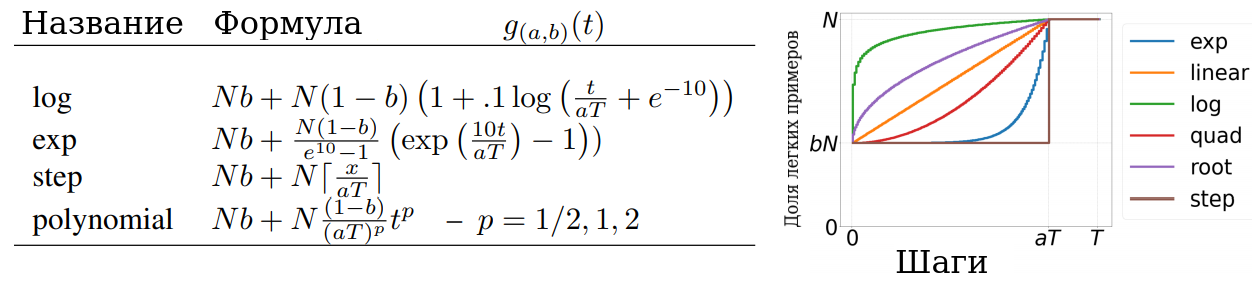
\includegraphics[scale=0.48]{CV_pacing_functions}
	\caption{Семейство функций для семплирования данных}
	\label{fig:cv_pacing_functions}
\end{figure}

\subsection{Применение обучения по плану в обработке естественного языка}
\ 

В обработке естественного языка существует ограниченное число существенных результатов в контексте применения обучения по плану. Вероятно, это связано с тем, что естественный язык состоит из слов и предложений, не имеющих строгую структуру, которую сложно формально описать. Более того, на данный момент наука не понимает всех процессов, происходящих внутри современных языковых моделей.

Platanios и др.~\cite{platanios2019competence} исследовали влияние обучения по плану на задаче машинного перевода на скосрость сходимости нейронных сетей. Авторы рассмотрели две метрики сложности текстов: длину и вероятность правдоподобия, которая вычисляется по формуле (\ref{eq:log_likelihood}), где $s_i$ -- текст или набор токенов, $w_k^i$ -- слово или токен, $p(x)$ -- доля токенов $x$ во всем датасете.

\begin{equation} \label{eq:log_likelihood}
d(s_i) = -\sum\limits_{k=1}^{N}\log p(w_k^i)
\end{equation}

Они показали, что правдоподобие не имеет никаких преимуществ по сравнению  с длиной с точки зрения скорости обучения моделей. В качестве семплеров был взят префиксный семплер с функцией $c(t)$ (формула (\ref{eq:competence_based_sampler})), вычисляющий долю простых примеров, доступных для построения батча.

\begin{equation} \label{eq:competence_based_sampler}
c(t) = \min\left(1, \sqrt{t\frac{1 - c_0^2}{T} + c_0^2}\right)
\end{equation}

$T$ -- общее число тренировочных шагов, $c_0$ -- доля простых примеров, доступных в самом начале обучения (авторы используют $c_0 = 0.01$)

В итоге, ученые добились улучшения качества модели на 2.2 BLEU и ускорения обучения на 70\%.

Xu и др.~\cite{xu2020curriculum} предложили альтернативный способ применения обучения по плану в обработке естественного языка на задаче Natural Language Understanding. Их метод оперирует понятием модельной оценки сложности текстов. Сложность примеров меняется в процессе обучения в зависимости от качества модели на момент применения метрики к примеру. Авторы предлагают алгоритм, который в цикле повторяет следующую процедуру. Тренировочный корпус данных разделяется на несколько частей. Затем, для каждого блока независимо обучается новая модель, которая инициализируется весами текущей глобальной модели. После этого оценивается сложность всех примеров как сумма уверенностей всех моделей по всем блокам кроме блока, в котором находится данный пример (рис. \ref{fig:acl20_algo_difficulty}).

\begin{figure}[h]
	\centering
	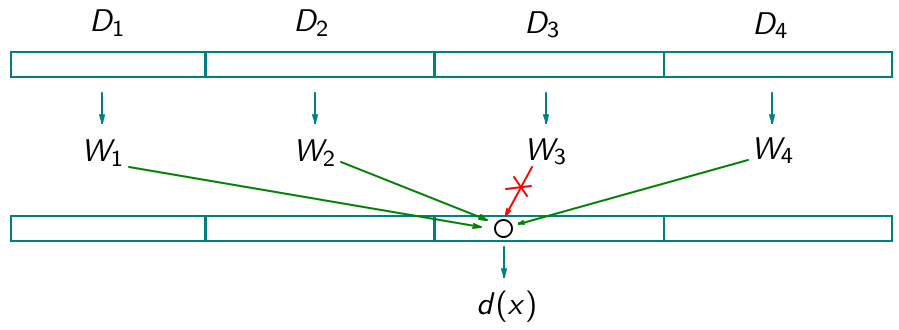
\includegraphics[scale=0.48]{acl20_algo_difficulty}
	\caption{Алгоритм вычисления модельной метрики сложности текста. На данной схеме датасет делится на $4$ части, на каждой из которых учится независимая модель BERT с началными весами текущей глобальной модели. Сложность примеров в блоке под номером $3$ вычисляется как сумма уверенностей моделей $W_1,W_2,W_4$.}
	\label{fig:acl20_algo_difficulty}
\end{figure}

Наконец, весь датасет сортируется в соответствии с найденными сложностями примеров, и текущая глобальная модель обучается на новой эпохе, обрабатывая примеры в порядке возрастания сложности. Данный подход позволяет улучшить точность итогвоой модели на 1.5\%, но требует существенно больше времени.

В 2017 году Kocmi и др.~\cite{kocmi2017curriculum} провели сравнтиельный анализ двух подходов к ускорению обучения: minibatch bucketing и обучение по плану. Первый подход отличается от стандартного алгоритма обучения нейронных сетей только построением батчей, каждый из которых содержит данные, слабо отличающиеся по заранее определенному показателю (например, батч из предложений с не более чем пятью глаголами). Для обучения по плану авторы используют три метрики.
\begin{enumerate}
	\item длина предложения
	\item максимальный частотный ранг слова -- для каждого слова вычисляется количество его вхождений в тренировочный корпус данных. Затем все слова сортируются в порядке убываения частоты. Рангом слова называется его позиция в данном отсортированном массиве. Сложность предложения определяется как максимальный ранг по всем словами в данном предложении
	\item количество конъюнкций (например, эту метрику можно определить как количество союзов)
\end{enumerate}

Исследование показало, что обучение по плану позволяет увеличить качество итоговой модели на 1 BLEU, но без уменьшения времени обучения. Более того, модель, обучаемая с помощью обучения по плану достигает 85\%-го качества модели, обученной базовым алгоритмом, в два раза медленнее.

Важный вклад в исследование обучения по плану внесли Zhang и др.~\cite{zhang2018empirical} в 2018 году. В качестве метрик оценки сложности текста авторы рассматривают модельную метрику, длину, максимальный частотный ранг и средний частотный ранг. В данной работе ранг слова определяется аналогично работе Kocmi и др.~\cite{kocmi2017curriculum}. Модельная метрика определяется ошибкой вспомогательной модели, заранее обученной на задачу машинного перевода стандартным алгоритмом. Принципиальным отличием данной работы является выбор методов построения батчей. Ученые не рассматривают префиксные семплеры, а используют алгоритмы, с течением времени изменяющие распределение вероятности взять пример в текущий батч. Авторы показали, что обучение по плану очень чувствительно к выбору гиперпараметров. Среди нескольких десятков конфигураций лишь некоторые позволяют получить ускорение обучения модели до 30\% без потери точности. Также было установлено, что длина не является удачной метрикой для обучения по плану, а именно она приводит к замедлению обучения модели до двух раз и уменьшению точности модели до 4.2 BLEU.

\subsection{Существующие метрики оценки сложности текстов}
\ 

Таким образом, был рассмотрен ряд метрик, активно используемых в обучении по плану: длина~\cite{platanios2019competence, kocmi2017curriculum, zhang2018empirical}, вероятность правдоподобия~\cite{platanios2019competence}, модельная~\cite{xu2020curriculum}, максимальный~\cite{kocmi2017curriculum, zhang2018empirical} и средний~\cite{zhang2018empirical} частотный ранг.

На первый взгляд кажется, что можно придумать еще несчетное количество подходов. Действительно, существует большое количество метрик оценки сложности текстов. Это показал Kurdi в своей статье 2020 года \cite{kurdi2020text}, в которой решал задачу определения уровня английского языка, необходимого для прочтения текста. Для этого он строил множество признаков входного текста для их передачи на вход классификатору. Ученый рассмотрел несколько десятков методов определения сложности текста понятных для человека: фонологические, морфологические, лексические, синтаксические признаки и многие другие. Это позволило решить задачу с высокой точностью. Несмотря на хорошее качество полученной модели, вопрос применимости данных метрик к обучению по плану остается открытым. Однако на него можно найти ответ в работе Frans van der Sluis и Egon L. van den Broek \cite{van2010using}. Они рассмотрели два набора данных, Wikipedia и Simple English Wikipedia (упрощенная версия Wikipedia, состоит из статей меньшей длины, написанных более простым языком), и показали что лингвистические метрики плохо коррелируют с реальной сложной текстов. Таким образом, классические методы оценки сложности текстовых данных имеют меньший приоритет для рассмотрения в сранении с метриками, основанными на статистических подходах.

Оценка сложности текстов тесно связана с количеством информации в них. Этот объкт изучает теория информации. В 2006 году Ay и др. \cite{ay2006unifying} предложили четыре метода оценки сложности конечных дискретных систем. К сожалению, в чистом виде данные подходы невозможно применить к текстам, так как они (подходы) получают на вход некоторую совместно распределенную случайную величину. Однако эти метрики можно  адаптировать, о чем будет рассказано в последующих главах.

\subsection{Выводы}

\begin{itemize}
	\item Нет существующих исследований влияния обучения по плану на скорость сходимости на не менее важных задачах предобучения языквоых моделей и классификаии текстов
	\item Рассмотрено узкое множество метрик оценки сложности текстов, которое можно расширить, используя методы из смежных областей математики и информатики, таких как теория информации и информационный поиск
	\item Большинство работ применяют обучение по плану для улучшения качества модели, но не скорости ее обучения
	\item Можно заметить, что во многих работах обучение по плану приводит к уменьшению тренировочного времени и увеличению точности моделей только в определенных конфигурациях, которые сильно зависят от гиперпараметров, задачи, модели и корпуса данных. Важной деталью является тот факт, что все эксперименты были проведены на чистых наборах данных. Такая ситуация редко встречается при решении прикладных задач и реализации реальных проектов. Например, крупные компании тратят большие деньги для очистки тренировочных данных. Таким образом, важность исследования обучения языковых моделей на шумных корпусах данных очевидна, однако работ, освещяющих данный вопрос найдено не было
\end{itemize}

\section{Метрики оценки сложности текстов}
\subsection{Описание метрик}
\ 

Одним из недостатков существующих работ является узкое множество рассматриваемых метрик. Чтобы решить эту проблему необходимо предложить ряд метрик, расширяющих это множество. В данной работе не рассматриваются линвгистические метрики, так как они плохо себя показали в существующих работах, рассмотренных в главе \ref{sec:literature}.

Во-первых, необходимо взять уже существующие методы оценки сложности текстов.
\begin{enumerate}
	\item Длина текста
	\item Вероятность правдоподобия (формула (\ref{eq:log_likelihood}))
	\item Максимальный частотный ранг
\end{enumerate}

Во-вторых, в рамках данной работы я предлагаю взглянуть на задачу оценки сложности текстов с точек зрения информационного поиска, теории информации и обучаемой модели.

Информационный поиск занимается быстрым поиском документов в большой базе данных по входному запросу. В простом описании это делается посредством поиска ближайшего документа по некоторому расстоянию (например, косиносному). Чтобы считать дистанцию, нужно по документу получить некоторый вектор. Одним из наболее популярных и простых способов это сделать является применение метрики TF-IDF (формула (\ref{eq:tf_idf})).

\begin{equation} \label{eq:tf_idf}
TF\_IDF(d,t) = TF(d,t)\cdot IDF(t,D)
\end{equation}

\begin{equation} \label{eq:tf}
TF(d,t) = \frac{n_t}{\sum\limits_{j}n_j}
\end{equation}

\begin{equation} \label{eq:idf}
IDF(t,D) = \frac{|D|}{|\{d\in D\colon t \in d\}|}
\end{equation}

Здесь $D$ -- коллекция документов, $d$ -- конкретный документ из коллекции, $t$ -- конкретный токен (слово в предложении) в документе. Таким образом TF\_IDF -- это произведение TF и IDF, где TF -- вероятность вхождения токена в документ, а IDF -- это величина, обратная доле документов, в которых встречается данный токен. Эта метрика максимизируется, когда частый токен в конкретном документе встречается в малой доле всех документов, следовательно она выделяет набиолее важные токены в документе. Заметим, что TF\_IDF позволяет получить по тексту некоторый вектор, а мы хотим получить некоторое число. Давайте рассмотрим сумму TF\_IDF по всем словам в предложении. Таким образом, мы определяем потенциал предложения как сумму важностей входящих в него слов.

Теория информация позволяет понять, сколько информации находится в том или ином объекте. Давайте рассмотрим универсальный фреймворк для измерения сложности конечных систем, предложенный Ay и др.~\cite{ay2006unifying}. Авторы заметили, что количество информации в дискретных последовательностях не является простой суммой количества информации в отдельных ее частях, и предложили четыре подхода, основанных на декомпозиции системы на подсистемы в контексте их иерархического взаимодействия. В чистом виде данные методы нельзя применить к текстам, так как они оперерируют понятием совместно распределенной случайной величины. Возьмем две метрики, одновременно содержательных и удобных для адаптации к задаче обработки естественного языка, а именно TSE (формула (\ref{eq:tse})) и Excess Entropy (EE, формула (\ref{eq:ee})).

\begin{equation} \label{eq:tse}
\begin{split}
	& TSE(X_V) = \sum\limits_{k=1}^{n-1}\frac{k}{n}C^{(k)}(X_V) \\
	& C^{(k)}(X_V) = \frac{n}{k\binom{n}{k}}\sum\limits_{A\subseteq V,|A|=k}H(X_A) - H(X_V)
\end{split}
\end{equation}

\begin{equation} \label{eq:ee}
EE(X_V) = \left[\sum\limits_{v\in V}H(X_{V\backslash\{v\}})\right] - (n - 1)H(X_V)
\end{equation}

Здесь $X_V = \left(X_1,X_2,\ldots,X_n\right)$, $V = \{1,2,\ldots,n\}$, $A=\{i_1,i_2,\ldots,i_k\}$, $X_A = \left(X_{i_1},X_{i_2},\ldots,X_{i_k}\right)$, $H$ -- энтропия, $n$ -- длина вектора $X$.

Теперь необходимо научиться их использовать, а именно по тексту $T=(t_1,t_2,\ldots,t_n)$ построить некоторую совместно распределенную случайную величину (вектор вещественнозначных случайных величин) $\xi$. Определим $\mu_i := \xi_{t_i}^{i}$ как бинарную (принимающую значения из $\{0, 1\}$) случайную величину, зависящую от значения слова $t_i$ в тексте и его позиции $i$. Пусть $P(\xi_{t_i}^i = 1) = \frac{\text{число текстов, у которых на } i \text{-й позиции стоит слово } t_i}{\text{общее число текстов длины хотя бы }i}$. Тогда $\xi = (\xi_{t_1}^1,\xi_{t_2}^2,\ldots,\xi_{t_i}^i,\ldots,\xi_{t_n}^n)$. Такая адаптация позволяет использовать теоретико-информационные метрики, сохраняет структуру предложения и учитывает статистические особенности конкретного примера относительно всего датасета.

Теперь рассмотрим подход, который будет опираться на показания обучаемой модели. Пусть мы тренируем модель $M_1$ типа $T$ (например, BERT). Возьем модель $M_2$ того же типа, заранее предобученную на задачу Masked Language Modelling (MLM). В процессе предобучения оптимизируется кросс энтропия. Определим сложность примера $T_i$ как значение данной функции потерь модели на данном примере (формула \ref{eq:mlm_loss})

\begin{equation} \label{eq:mlm_loss}
MLM\_loss(T_i) = CrossEntropy(T_i, M_2(T_i))
\end{equation}

Здесь $M_2(T_i)$ -- предсказание модели $M_2$ после замены 15\% случайных слов на пробелы.

Заметим, что такой подход опирается на структуру конкретной модели и позволяет косвенно определить, насколько конкретный пример сложен для рассматриваемой модели. Данная метрика мотивирована существующими аналогами из рассмотренных в главе \ref{sec:literature} работ.

Одно из направлений исследований, представленных в данной работе, а именно обучение на шумных тренировочных данных позволило выявить метрику, которая дает положительные результаты в контексте применения обучения по плану. Рассмотрим величину, равную среднему числу токенов на слово. Более формально этот подход описывается следующим образом.

\begin{itemize}
	\item На вход рассматриваемой в данной работе модели BERT подается последовательность токенов, полученная применением токенизатора к входному тексту
	\item Таким образом, мы знаем количество слов в тексте $w$ и число токенов $t$ в полученной последовательности токенов
	\item Определим среднее число токенов на слово как $TPW=\frac{t}{w}$ (tokens per word)
\end{itemize}

Данный подход возник после проведения экспериментов, заключающихся в обучении модели на шумном наборе данных (тексты с опечатками), и наблюдении за данными, которые подаются на вход модели. Выяснилось, что шумный текст токензируется большим числом токенов, так как словарь токенизатора состоит в основном из наиболее частых слов в языке. Шумный же набор данных состоит из слов со множеством опечаток, что не позволяет обойтись малым число токенов на слово. Таким образом данная метрика позволяет отсортировать данные в порядке зашумленности. Другими словами в начале обучения модель будет учиться на чистых примерах, постепенно переходя к предложениям с большим числом опечаток, что приводит к более стабильному обучению.

\subsection{Алгоритмы вычисления метрик}
рассмотреть все метрики,сказать за какую асимптотику можно посчитать,если нужно, описать алгоритм и привести сравнительную таблицу реального времени работы,описать все статистики,которые нужно собрать,

Перейдем к описанию алгоритмов вычисления предложенных метрик. Обратимся к таблице \ref{table:def_metrics_asymptotics} 

\begin{table}[h]
	\label{table:def_metrics_asymptotics}
	\caption{Время работы алгоритмов вычисления метрик по определнию на корпусе данных из не более 10 миллионов текстов длины меньше 500}
	\centering
	\begin{tabular}{|l|c|c|}
		\hline
		Метрика & Асимптотика & Реальное время работы \\
		\hline
		Длина & $\mathcal{O}(n)$ & < 30 мин. \\
		Вероятность правдоподобия & $\mathcal{O}(n)$ & < 5 ч.\\
		Максимальный частотный ранг & $\mathcal{O}(n)$ & < 5 ч. \\
		\hline
		TF-IDF & $\mathcal{O}(n)$ & < 5 ч. \\
		\hline
		TSE & $\mathcal{O}^*(2^n)$ & {\bf $\infty$} \\
		EE & $\mathcal{O}(n^2)$ & > 1 мес. \\
		TPW & $\mathcal{O}(n)$ & < 5 ч. \\
		\hline
	\end{tabular}
\end{table}

Видно, что большинство метрик не нуждаются в разработке производительного алгоритма для их вычисления. Однако, для TSE и EE это сделать придется.

Сначала разберем алгоритм вычисления энтпроии у вектора большой длины. Распишем энтропюию как сумму условных энтропий. Также предположим, что достаточно далекие друг от друга случайные величины независимы. Получим формулу~ \ref{eq:h_mu_sum_cond_h}.

\begin{equation} \label{eq:h_mu_sum_cond_h}
H(\mu) = \sum\limits_{i=1}^{n}H(\mu_i|\mu_1,\mu_2,\ldots,\mu_{i-1}) = \sum\limits_{i=1}^{n}H(\mu_i|\mu_{i-L},\ldots,\mu_{i-1})
\end{equation}

Здесь $L$ -- это длина контекста, от которого будет зависеть случайная величина~$i$. Заметим, что при выборе достаточно большого контекста энтропия ввыродится в длину, так как можно считать, что все подтексты длины $L$ разные, следовательно вероятность того, что $\mu_1=x_1,\mu_2=x_2,\ldots,\mu_L=x_L$ одинакова для всех $(x_1,\ldots,x_L)$, которые встречаются в датасете. Однако в процессе реализации вычисления энтропии выяснилось, что даже при $L = 2$ время работы существенно превышает итоговое время обучения модели. Таким образом, приходится ограничиваться случаем $L=1$. В итоге получаем формулу (\ref{eq:entropy}) для вычисления энтпроии, каждое слагаемое в котором вычисляется за $\mathcal{O}(1)$.

\begin{equation} \label{eq:entropy}
H(\mu) = H(\mu_1) + H(\mu_2|\mu_1) + \ldots + H(\mu_i|\mu_{i-1}) + \ldots + H(\mu_n|\mu_{n-1})
\end{equation}

Разберем алгоритм вычисления метрики EE. Заметим, что EE представляет из себя разность двух величин (формула (\ref{eq:ee})), последня из которых вычисляется за $\mathcal{O}(n)$. Необходимо соптимизировать вычисление первой величины $\sum\limits_{v\in V}H(X_{V\backslash\{v\}})$. Раскроем $H(X_{V\backslash\{v\}})$ по формуле (\ref{eq:entropy}), подставим это выражение в определение EE (формула (\ref{eq:ee})) и получим упрощенную версию формулы для EE, вычисляемую за $\mathcal{O}(n)$ (формула~(\ref{eq:ee_simplify})).

\begin{equation} \label{eq:ee_simplify}
\begin{split}
& \sum\limits_{i=1}^{n}H(\mu_1,\ldots,\mu_{i-1},\mu_{i+1},\ldots,\mu_n) =
\sum\limits_{i=1}^{n}H(\mu) - H(\mu_i|\mu_{i-1}) - H(\mu_{i+1}|\mu_i) + H(\mu_{i+1}) \\
& EE(X) = \sum\limits_{i=2}^{n}H(\mu_i) - H(\mu_i|\mu_{i-1})= \sum\limits_{i=2}^{n}I(\mu_{i-1}\colon\mu_i)
\end{split}
\end{equation}

Наконец, разберем алгоритм вычисления TSE. Данную метрику можно вычислить за экспоненциальное время, но для этого нужны огромные ресурсы. Первый разработанный мною алгоритм, вычисляющий TSE, работал за $\mathcal{O}(n^2)$. Он основывался на технике динамического программирования, однако он сложен для понимания и все еще требовал большого количства ресурсов. Однако позже был придуман алгоритм, работающий за $\mathcal{O}(n)$ и использущий разумное количество процессорного времени. Давайте опишем его в деталях.

Пусть $S_1 = \sum\limits_{i=1}^{n}H(\mu_i)$, $S_2 = \sum\limits_{i=2}^{n}H(\mu|\mu_{i-1})$, $h = H(X_V)$. Заметим, что $S_1,S_2,h$ вычисляются за $\mathcal{O}(n)$. В определении TSE фигурирует величина. Пусть $E = \frac{1}{\binom{n}{k}}\sum\limits_{A\subseteq V,|A|=k}H(\mu_A)$. Тогда $C^{(k)}(\mu_V) = \frac{n}{k}E - h$. Заметим, что $E$ -- математическое ожидание энтропии случайного подмножества случайных величин из множества $\{\mu_1,\ldots,\mu_n\}$. Воспользуемся линейностью математического ожидания и получим формулу (\ref{eq:E_lin}).

\begin{equation} \label{eq:E_lin}
E = \sum\limits_{i=1}^{n}A_iH(\mu_i) + \sum\limits_{i=2}^{n}B_iH(\mu_i|\mu_{i-1})
\end{equation}

Заметим, что $A_i$ -- вероятность того, что в случайном подмножестве будет $\mu_i$, но не будет $\mu_{i-1}$. Тогда $A_i$ вычисляются по формуле (\ref{eq:TSE_A_i}).

\begin{equation} \label{eq:TSE_A_i}
A_i = 
\begin{cases}
\binom{n-2}{k-1}/\binom{n}{k}=\frac{k(n-k)}{n(n-1)},& i > 1 \\
\binom{n-1}{k-1}/\binom{n}{k}=\frac k n,& i = 1
\end{cases}
\end{equation}

Аналогично, $B_i$ -- вероятность того, что и $\mu_i$, и $\mu_{i-1}$ будут в случайном подмножестве. Тогда $B_i$ вычисляются по формуле (\ref{eq:TSE_B_i}).

\begin{equation} \label{eq:TSE_B_i}
B_i = \frac{\binom{n-2}{k-2}}{\binom{n}{k}} = \frac{k(k-1)}{n(n-1)}
\end{equation}

Заметим, что $\forall i > 2$ верно $A_i = A_2$ и $\forall i$ верно $B_i = B_2$. Тогда верна формула (\ref{eq:TSE_E_final}).

\begin{equation} \label{eq:TSE_E_final}
E = A_1H(\mu_1) + A_2(S_1 - H(\mu_1)) + B_2S_2
\end{equation}

Таким образом, итоговый алгоритм вычисляет TSE за линейное время и требует пренебрежимо маленькое количество времени по сравнению со всем временем обучения модели.

\subsection{Сбор статистик}
\ 

Для вычисления большинства метрик требуются дополнительные статистики, собираемые со всего датасета.

\begin{itemize}
	\item длина $\rightarrow$ число текстов с такой длиной
	\item $(i, x_i) \rightarrow$ число текстов, где $t_i = x_i$ 
	\item $(x_i)\rightarrow$ число текстов, где $x_i$ является последним токеном
	\item $(i, x_{i-1}, x_i) \rightarrow$ число текстов, где на $(i-1)$-й позиции стоит $x_{i-1}$, а на $i$-й позиции стоит $x_i$
	\item $x_i \rightarrow$ число текстов, в которых есть $x_i$
	\item $x_i \rightarrow $ число вхождений $x_i$ в весь датасет
\end{itemize}

На больших датасетах тривиальный алгоритм сбора таких статистик может занимать большое количество времени, так как при росте размера корпуса данных количество ключей в хранилище также возрастает, что приводит к замедлению системы. Поэтому был предложен алтернативные подход. Заметим, что все статистики не трубуют информации от двух предложений в один момент времени. Тогда можно поделить весь датасет на несколько блоков, собрать статистики на каждом из них, а после слить в одно хранилище. Этот способ ускоряет подсчет статистик в несколько десятков раз, так как количество ключей при подсчете одного блока небольшое, следовательно и сбор данных из одного куска, и слияние всех статистик в одно место требуют значительно меньше ресурсов.

\begin{table}[h]
	\label{table:collect_stats_time}
	\caption{Время работы алгоритмов сбора статистик на корпусе данных из не более 10 миллионов текстов длины меньше 500}
	\centering
	\begin{tabular}{|c|c|}
		\hline
		Режим & Реальное время работы \\
		\hline
		1 CPU & $\approx$ 2 недели \\
		5 CPU & $\approx$ 1-2 дня \\
		20 CPU & < 6 ч. \\
		\hline
	\end{tabular}
\end{table}

Таким образом, при делении корпуса данных примерно на 20 равных частей можно собрать все необходимые статистики за разумное время.
\pagebreak
\subsection{Выводы}
\ 

В этой главе мною был предложен ряд метрик оценки сложности текстов из разных областей математики и информатики: длина, вероятность правдоподобия, максимальный ранг слова, TF-IDF, EE, TSE, TPW. Метрики EE и TSE были адаптированы под задачу обработки естественного языка. Для всех метрик был описан линейный алгоритм их вычисления, требующий пренебрежимо маленькое количество временных ресурсов относительно общего времени обучения. Также был представлен производительный алгоритм сбора статистик, необходимых для вычисления предложенных метрик.

\section{Конфигруация экспериментов}
Описать, что будет происходить в главе (после написания самой главы)
\subsection{Алгоритмы семплирования}
описать все готовые семплеры с обозначением, сказать, что они сделаны не мной
\subsection{Данные}
рассказать про корпуса данных (BookCorpus,sentiment140,Hyperpartisan News Detection)
\subsection{Метод сравнения метрик}
Рассказать, как будут сравниваться две метрики на предмет скорости обучения модели
\subsection{Выводы}
\section{Эксперименты}
Описать, что будет происходить в главе (после написания самой главы)
\subsection{Влияние обучения по плану на задаче предобучения}
\subsection{Влияние обучения по плану на задаче классификации}
\subsection{Влияние обучения по плану на шумном корпусе данных}
\subsection{Выводы}
\section*{Заключение}

% размещенный с предпочтением "вверху страницы"
% \begin{figure}[t]
% \centering
% 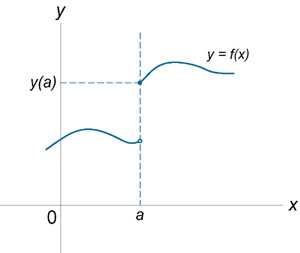
\includegraphics{fig1.jpg}
% \caption{Разрыв функции}
% \label{разрыв_функции}
% \end{figure}

% \begin{figure}[h]
    % 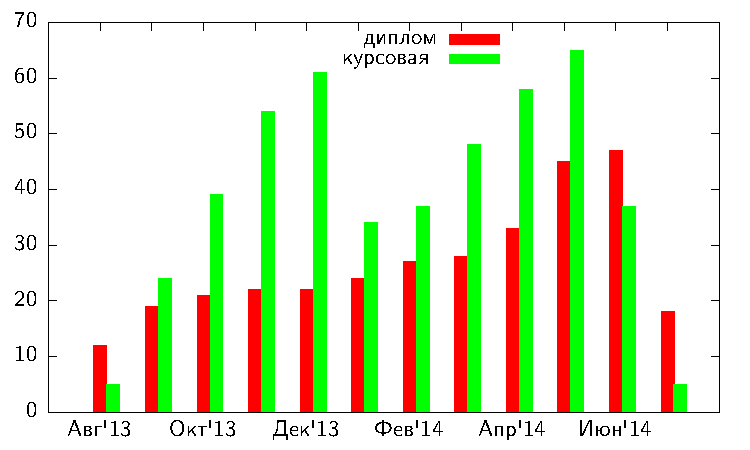
\includegraphics{thesis-search-trends}
    % \caption{Статистика поисковых запросов в течении года}
% \end{figur

\bibliographystyle{ugost2008ls}
\bibliography{diploma.bib}
\end{document}
